
\documentclass[12pt]{amsart}
\usepackage{geometry} % see geometry.pdf on how to lay out the page. There's lots.
\usepackage{graphicx}
\usepackage{amsmath}
\geometry{letterpaper} % or letter or a5paper or ... etc
% \geometry{landscape} % rotated page geometry
\usepackage{fancyhdr} % This should be set AFTER setting up the page geometry
\pagestyle{fancy} % options: empty , plain , fancy
\renewcommand{\headrulewidth}{0pt} % customise the layout...
\lhead{}\chead{}\rhead{}
\lfoot{}\cfoot{}\rfoot{\thepage}
% See the ``Article customise'' template for come common customisations

\title{Numerical Simulation of Heat Flow in a Rod and Heat-Sensitive Fluid Bath}
\author{}
\date{} % delete this line to display the current date

%%% BEGIN DOCUMENT
\begin{document}

\maketitle
\section{Task 1}
\subsection{Numerical Method}
The equation governing the temperature in the rod is given as
\begin{equation}
\frac{\delta T}{\delta t} - \alpha \frac{\delta^2 T}{\delta x ^2} = Q(x,t)
\label{eq:begin}
\end{equation}
Where $Q(x,t)$ is the heat source function in terms of x and t.\\
This equation is a parabolic partial difference equation because it has both a spatial and time dependent component. This is not a steady state problem so we must discretize both the spatial and time components. In this case, we require approximations of the second derivative in space and the first derivative in time. An explicit forward finite difference method was chosen for this simulation because the initial temperature distribution of the rod is known. 
While implicit methods often offer faster convergence, they require additional data points to be solved simultaneously, which was determined to be beyond the scope of this simulation. \\
The second order spatial partial derivative is approximated as a center-divided finite difference, which introduces an error of $O((\Delta x)^2
)$. The first order time partial derivative is approximated as a forward finite-divided differnece, which introduces an error of $O(\Delta t)$. Refer to Section \ref{stabilitycriteria} for discussion of the selection of $\Delta x$ and $\Delta t$. 
\subsection{Equations Used}

The finite difference method uses the following approximations for the partial derivatives:
\begin{equation}
\frac{\delta T}{\delta t} = \frac{T^{l+1}_i - T^l_i}{\Delta t}
\label{eq:dTdtapprx}
\end{equation}

\begin{equation}
\frac{\delta^2 T}{\delta x^2} = \frac{T^l_{i+1} - 2T^l_i + T^l_{i-1}}{\Delta x^2}
\label{eq:dTdxapprx}
\end{equation}

Note that in the approximations shown in Equations \ref{eq:dTdtapprx} and \ref{eq:dTdxapprx} use a discretized step size (either $\Delta t$ or $\Delta x$) in order to convert from the exact solution to an approximation. \\
Substituting equations \ref{eq:dTdtapprx} and \ref{eq:dTdxapprx} into \ref{eq:begin} and solving for the $T^{l+1}_i$ term yeilds:

\begin{equation}
T^{l+1}_i = \Delta t Q(x,t) + \frac{\alpha \Delta t}{\Delta x^2} T^l_{i+1}+ (1-2\frac{\alpha \Delta t}{\Delta x^2}) T^l_i + \frac{\alpha \Delta t}{\Delta x^2} T^l_{i-1}
\label{eq:finitediff}
\end{equation}

Where l is the time index and i is the spatial index. 
\subsection{Stability Criteria} \label{stabilitycriteria}
The stability and convergence of the explicit finite difference method are dependent on the step size in both spatial and temporal dimensions, as well as the constants in the system. The stability criterion can generally be written as:

\begin{equation}
\lambda <= \frac{1}{2}
\label{eq:stabilitycondition}
\end{equation}

Based on the derivation used to calculate the approximation, we can modify this condition to:

\begin{equation}
\Delta t <= \frac{1}{2} \frac{\Delta x ^2}{\alpha}
\label{eq:stabilitystepsize}
\end{equation}

In this code, the $\Delta x$ was used to calculate the necessary $\Delta t$ in order to maintain stability. \\
Stability does not necessarily mean convergence, and Equation \ref{eq:stabilitycondition} can result in oscillatory solution. In order to reduce this possibility, one can modify Equation \ref{eq:stabilitycondition}  to 
\begin{equation}
\lambda <= \frac{1}{4}
\label{eq:stableconvergentcondition}
\end{equation}

This results in a time step size defined as:

\begin{equation}
\Delta t <= \frac{1}{4} \frac{\Delta x ^2}{\alpha}
\label{eq:stabilityconvergentstepsize}
\end{equation}

\subsection{Boundary and Initial Conditions}
The boundary conditions given are:
\begin{displaymath}
T(x=0,t) = 0
\end{displaymath}
\begin{displaymath}
T(x=L,t) = 300
\end{displaymath}
These boundary conditions imply that the temperature at each end of the rod is fixed throughout the simulation.\\
The initial conditions given are:
\begin{displaymath}
T(x, t=0) = 300
\end{displaymath}
\begin{displaymath}
\Theta(t=0) = 300
\end{displaymath}
The first initial condition states that the rod has a uniform initial temperature of 300. The second initial condition states that the heat-sensitive liquid has the same initial temperature. 

\section{Task 2: Solving Temperature Distribution in Rod}
The finite difference method was used, as described above, to solve for the temperature distribution in the rod as a function of t. At time t = 1.2 seconds, the temperature distribution is shown in Figure \ref{fig:tempdistat12s}. Note that the temperature axis in Figure \ref{fig:tempdistat12s} has been truncated to visualize the temperature variations along the rod. The resulting maximum temperature is 300.597 degrees, which occurs at x = 0.44. The parameters used to generate this approximation are listed in Table  \ref{task2param}.
\begin{center}
\begin{figure}
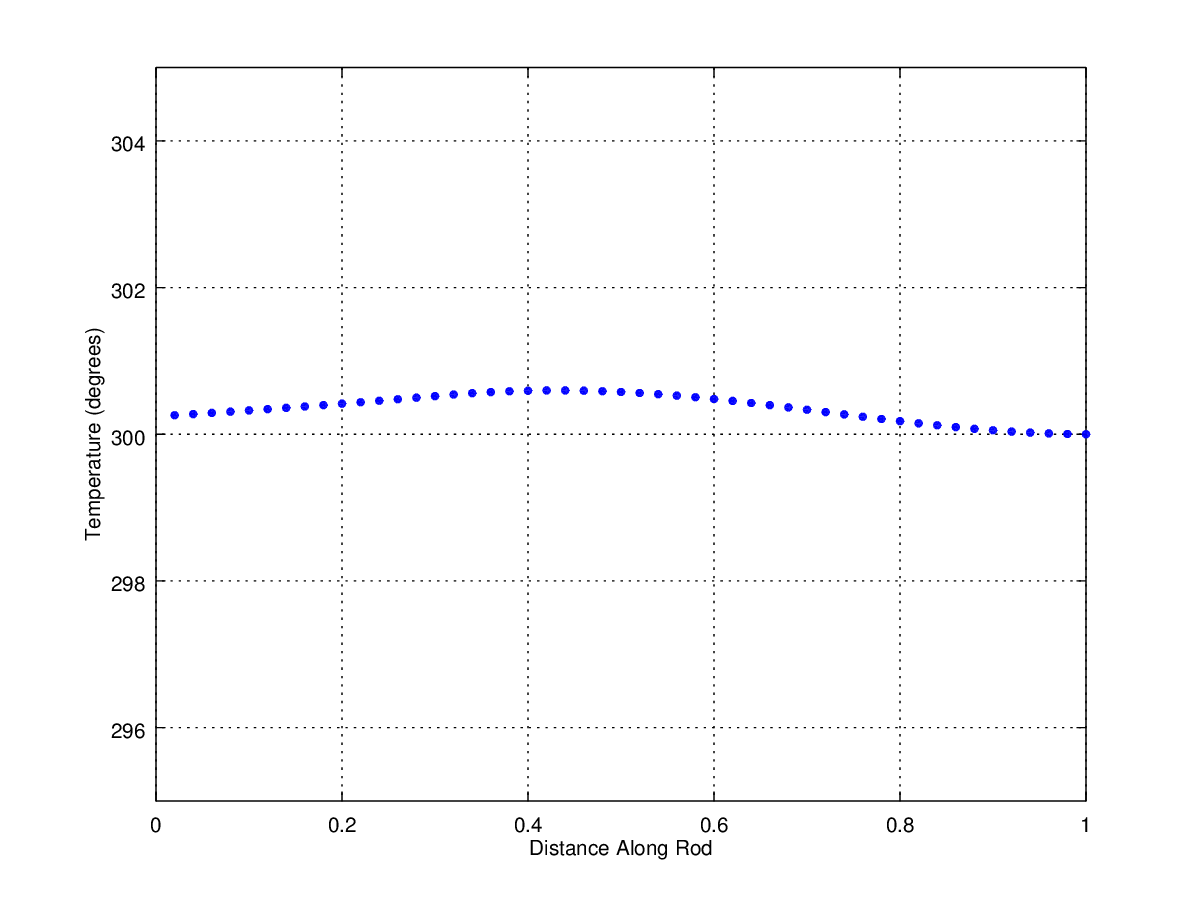
\includegraphics[scale=0.7]{task2fig}
\caption{Temperature Distribution Along Rod at t = 1.2 second}
\label{fig:tempdistat12s}
\end{figure}
\end{center}

\begin{table}[]
\centering
\caption{Task 2 Simulation Parameters}
\label{task2param}
\begin{tabular}{ll}
Parameter            & Value \\
$\Delta x$           & 0.02  \\
$\Delta t$           & 0.001 \\
Number of time steps & 127 \\
Error & $ O(0.0014)$
\end{tabular}
\end{table}

\section{Task 3: Temperature Evolution in Time} \label{tempevolutionsection}
Figure \ref{fig:task3fig} shows the changing temperature profile along the rod as a function of time at every second. Note that the points for t = 0, 1, 2, and 3 overlap. Variation in temperature is only evident after 3 seconds, when the profile becomes more defined. The evolution of this profile is limited in Figure \ref{fig:task3fig} due to the size of the plotted time steps- if we were to plot every 0.1 seconds, the evolution would be more defined. 
\begin{center}
\begin{figure}
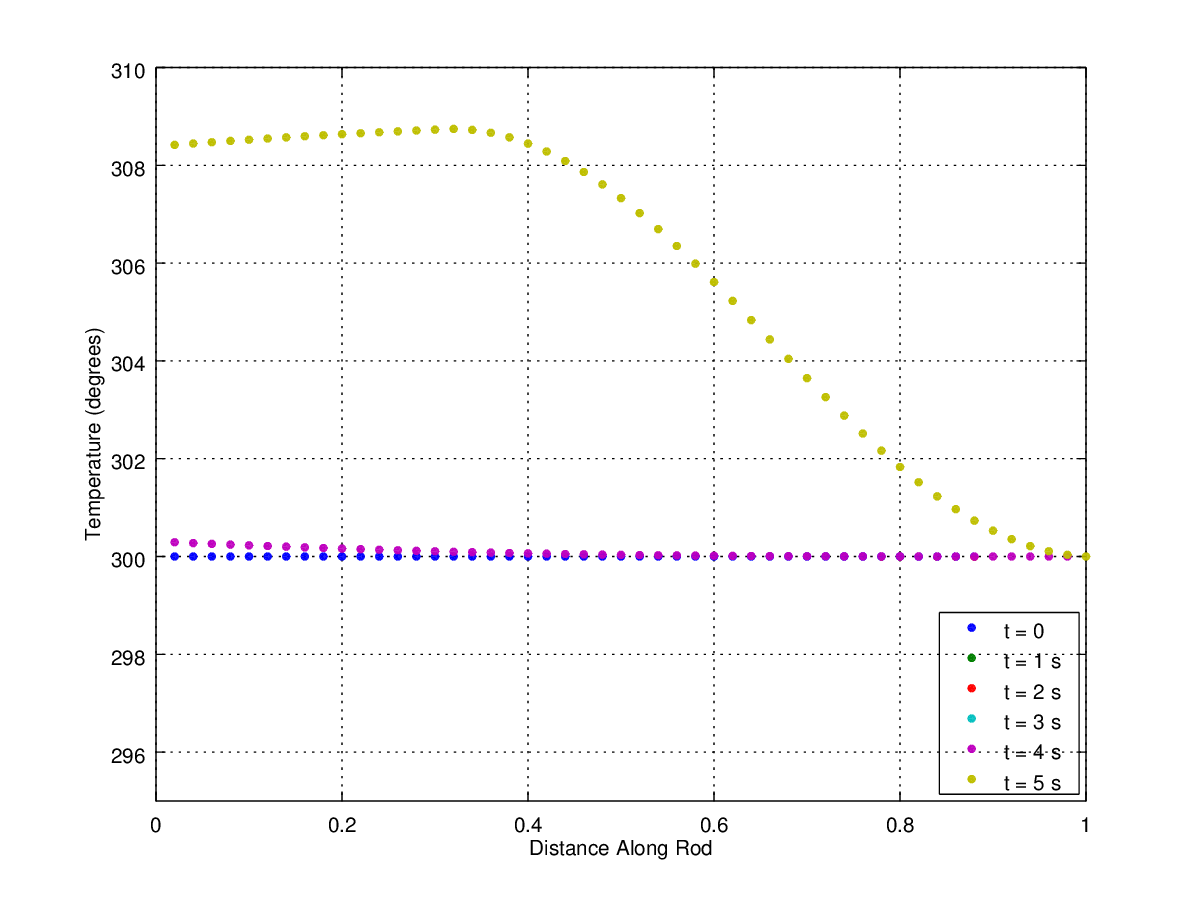
\includegraphics[scale=0.7]{task3fig}
\caption{Temperature Evolution Along Rod}
\label{fig:task3fig}
\end{figure}
\end{center}

\section{Task 4: Cubic Spline Interpolation of Maximum Temperature Data}

\subsection{Sampled Data} \label{datasamplesection}
The results of Section \ref{tempevolutionsection} were used to find the maximum temperature in the rod at each time step. This data was then sampled at every 0.4 seconds. The results of this sampling are shown in Figure \ref{fig:maxtempsamples}.

\begin{center}
\begin{figure}
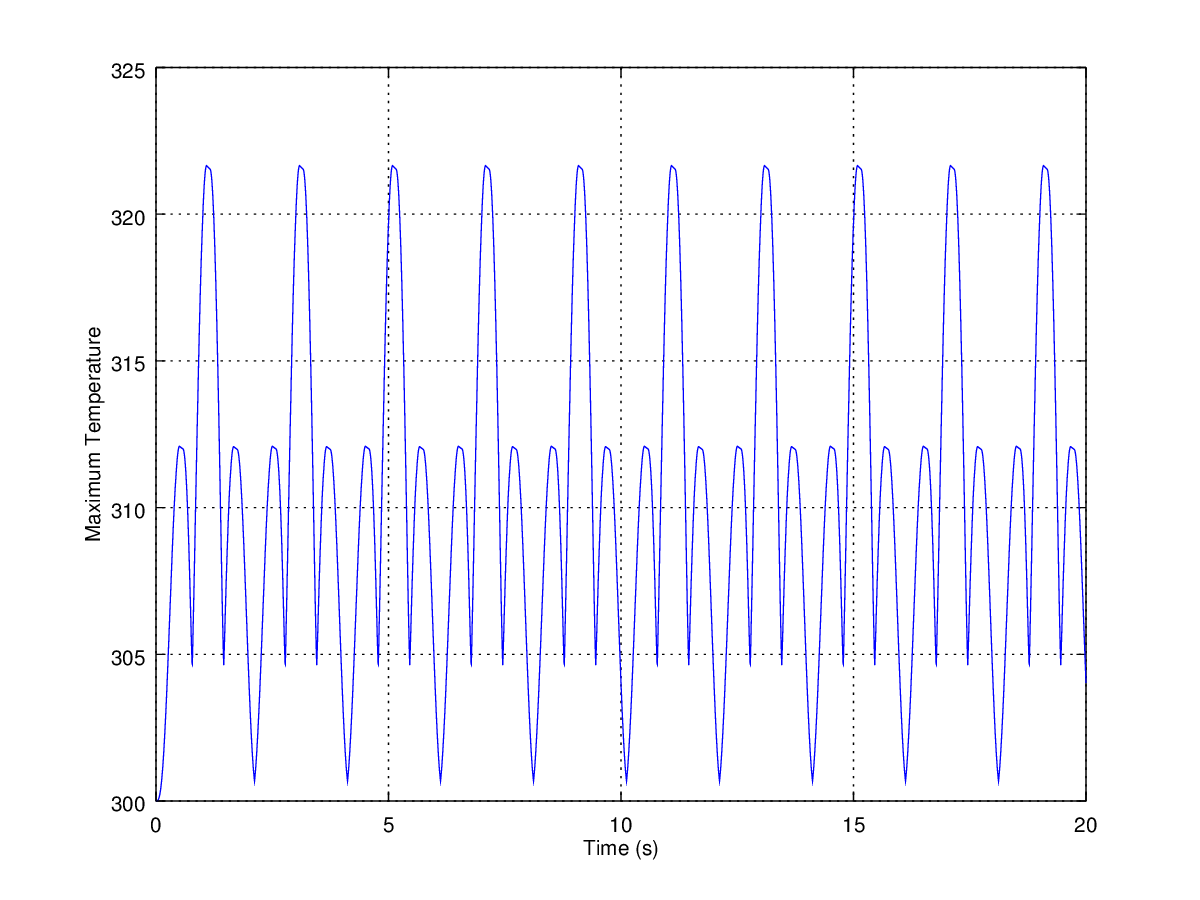
\includegraphics[scale= 0.7]{task4fig1}
\caption{Maximum Temperature Data Sampled Every 0.04 s}
\label{fig:maxtempsamples}
\end{figure}
\end{center}

\subsection{Cubic Spline Method}
The first task in calculating a cubic spline is to approximate the second derivatives using Equation \ref{eq:ddf}. Note that in this formulation, x represents the time variable, while f represents the maximum temperature. Equation \ref{eq:ddf} is applied twice, once as $x_i$ and once at $x_{i+1}$, to generate a system of 2 simultaneous equations with 2 unknowns. This process is repeated for all points in the vector to be approximated, and resulting $f''$ values are stored in a matrix. 

\begin{multline}
2(x_{i+1}-x_{i-1})f''(x_i) + (x_{i+1}-x_i)f''(x_{i+1})=\frac{6}{x_{i+1}-x_i} [ f(x_{i+1}) - f(x_i)] + \\ \frac{6}{x_i- x_{i-1}}[f(x_{i-1}) - f(x_i)]-(x_i-x_{i-1})f''(x_{i-1})
\label{eq:ddf}
\end{multline}

 Once the vector of second derivatives is calculated, the cubic spline approximation at each point x can be generated by applying Equation \ref{eq:splineapprxeq} at each desired x. 
\begin{multline}
f_i(x) = \frac{f''_i(x_{i-1})}{6(x_i - x_{i-1})}(x_i - x)^3 + \frac{f''_i(x_{i})}{6(x_i - x_{i-1})}(x - x_{i-1})^3+ \big[\frac{f(x_{i-1})}{x_i-x_{i-1}} - \frac{f''(x_i)(x_i-x_{i-1})}{6} \big](x_i - x) + \\ \big[\frac{f(x_{i})}{x_i-x_{i-1}} - \frac{f''(x_i)(x_i-x_{i-1})}{6} \big](x-x_{i-1})
\label{eq:splineapprxeq}
\end{multline}

\subsection{Results}
Figure \ref{fig:cubicspline} shows the maximum temperature as a function of time. It includes the original data from the simulation generated in previous sections, the sampled data in Section \ref{datasamplesection}, and the cubic spline interpolation based on this sample data. For the first several seconds, the cubic spline interpolation does a reasonably good job estimating the true (simulation) data. Around 8 seconds, the cubic spline misses a significant fluctuation in the maximum temperature, and it begins to fail significantly just beyond 16 seconds. This error could likely be reduced by increasing the number of sampled points that are used to generate the spline. These additional points would provide finer resolution for the spline algorithm, and thus increase the interpolation's accuracy. 
\begin{center}
\begin{figure}
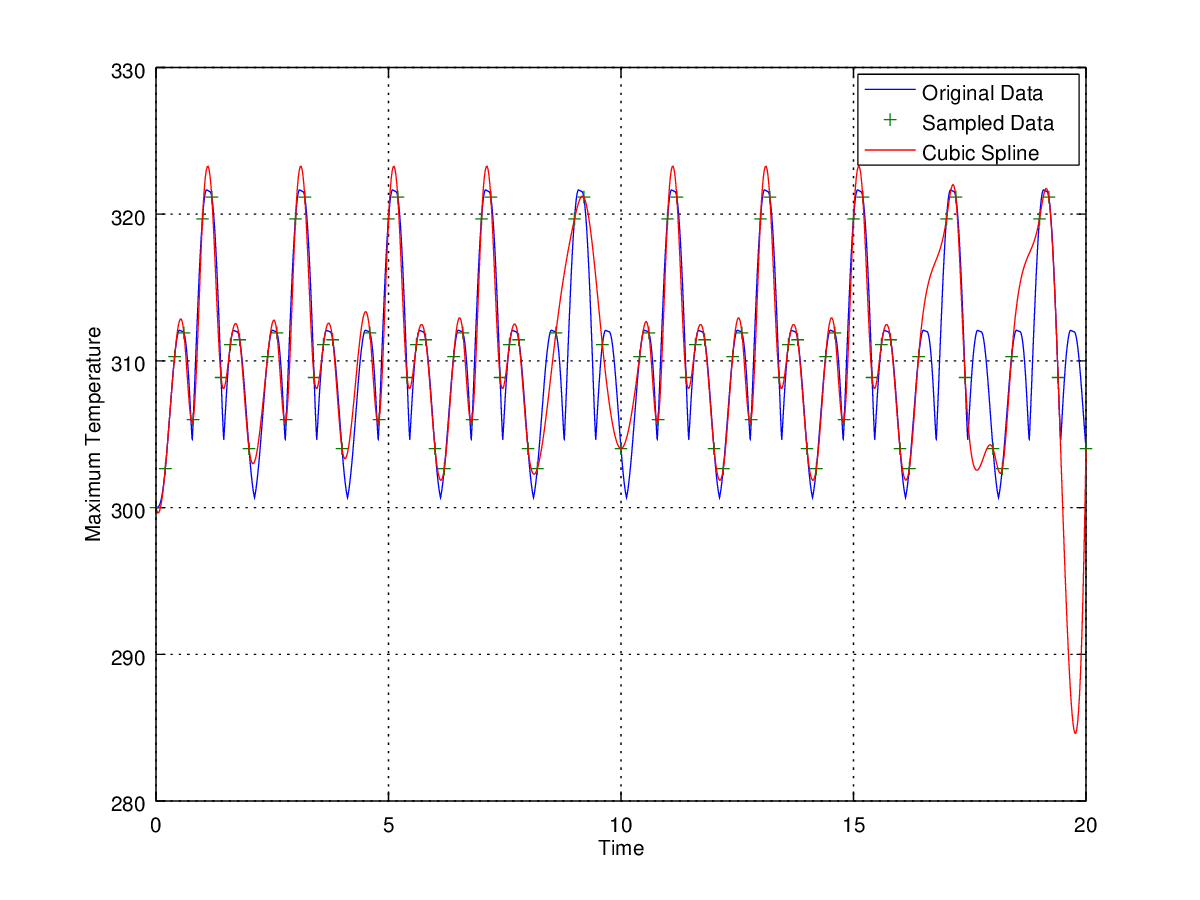
\includegraphics[scale=0.7]{task4fig2}
\caption{Maximum Temperature Data}
\label{fig:cubicspline}
\end{figure}
\end{center}

\section{Task 5: Heat Flow} \label{heatflowsection}
The heat flow as a function of time is given by
\begin{equation}
q(t) = \frac{\delta T}{\delta x}(x=0,t) 
\end{equation}
This first order partial derivative can be approximated by using a finite forward difference, as shown in Equation \ref{eq:qapprx}. 
\begin{equation}
\label{eq:qapprx}
\frac{\delta T(x,t)}{\delta x} = \frac{T^l_{i+1} - T^l_i}{\Delta x}
\end{equation}
Where the superscript $l$ refers to the lth time step and the subscript i refers to the ith spatial step.
Since the heat flow equation specifies that this heat flow occurs at x = 0, we can modify Equation \ref{eq:qapprx} to
\begin{equation}
\frac{\delta T(0,t)}{\delta x} = \frac{T^l_{1} - T^l_0}{\Delta x}
\end{equation}
Thus, we can iterate over all time steps to find the heat flow using Equation \ref{eq:qiter}. 
\begin{equation}
\label{eq:qiter}
q(t) = \frac{T^l_{1} - T^l_0}{\Delta x}
\end{equation}

Using this approximation, the heat flow was estimated for each time step in the simulation. This heat flow is shown versus time in Figure \ref{fig:q}.

\begin{center}
\begin{figure}
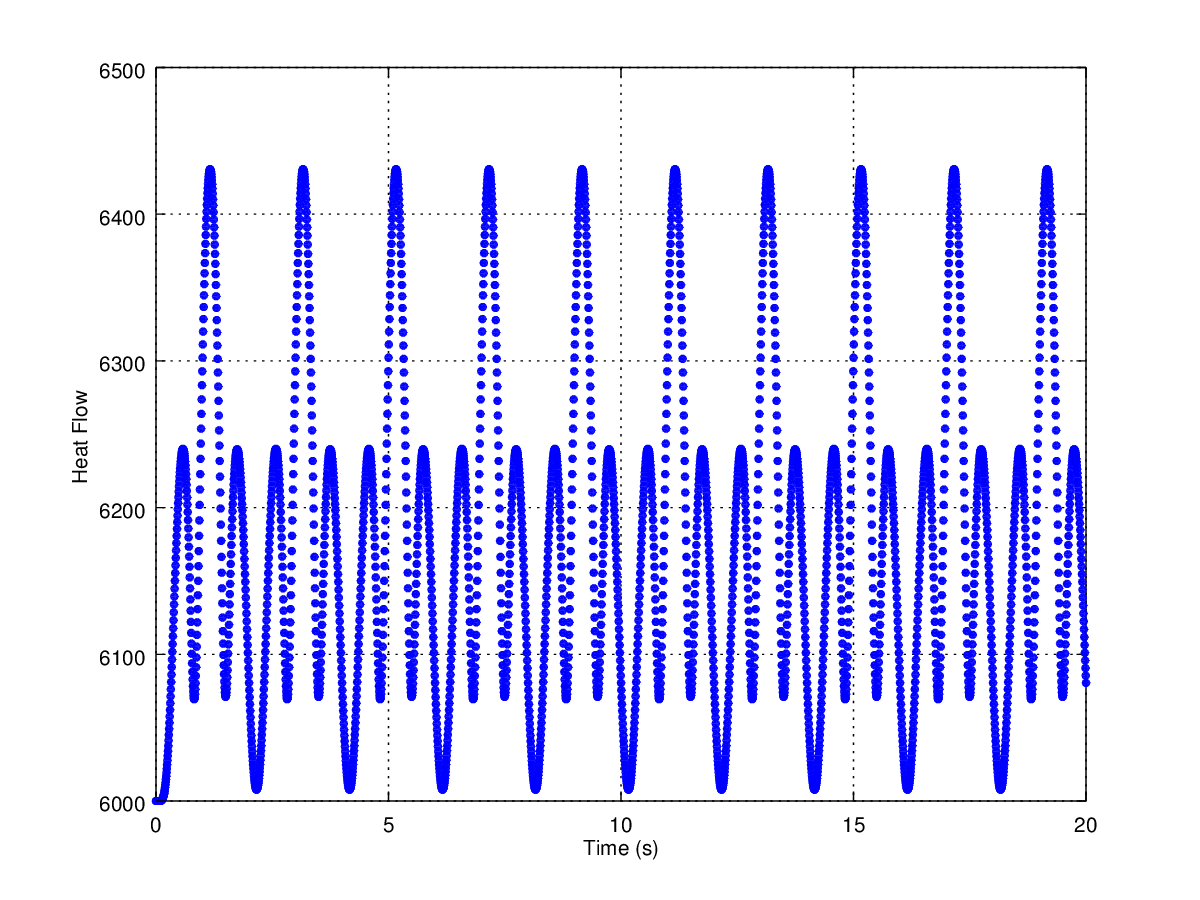
\includegraphics[scale=0.7]{task5fig}
\caption{Heat Flow Over Time}
\label{fig:q}
\end{figure}
\end{center}


\section{Task 6: Determining Maximum Temperature of Fluid} \label{fluidtempsection}
\subsection{Approximation Method}
The equation given for the temperature of the fluid as a function of time is
\begin{equation}
\frac{d \Theta}{dt}+ \beta (\Theta - 300)^2 = q(t)
\label{eq:thetaeq}
\end{equation}

See Section \ref{heatflowsection} for derivation of the approximation of $q(t)$. Using a forward finite difference approximation, Equation \ref{eq:thetaeq} can be approximated as

\begin{equation}
\frac{\Theta^{l+1} - \Theta^{l}}{\Delta t} + \beta (\Theta^l - 300)^2 = \frac{T^l_{i+1} - T^{l}_i}{\Delta x}
\label{eq:thetapprx}
\end{equation}
Where l is the time index and i is the spatial index. Recall from Section \ref{heatflowsection} that the heat flow equation is defined at the first two spatial nodes. Equation \ref{eq:thetapprx} can be solved to find theta at the next time step.

\begin{equation}
\Theta ^{l+1} = \Theta ^l - \beta \Delta t (\Theta ^l - 300)^2 + \frac{\Delta t}{\Delta x} T^l_2 - \frac{\Delta t}{\Delta x} T^l_1
\label{eq:thetaiter}
\end{equation}

\subsection{Simulation Results}
Equation \ref{eq:thetaiter} was used to approximate the time evolution of the liquid temperature from $0<=t<=20$ using the simulation parameters listed in Table \ref{task6param}. The resulting maximum temperature is 1100.866. 
\begin{table}[]
\centering
\caption{Task 6 and 7 Simulation Parameters}
\label{task6param}
\begin{tabular}{ll}
Parameter            & Value \\
$\Delta x$           & 0.05  \\
$\Delta t$           & 0.00625 
\end{tabular}
\end{table}

\section{Task 7: Plotting Fluid Temperature}
Using the simulation parameters described in Section \ref{fluidtempsection}, the temperature evolution of the fluid is shown in Figure \ref{fig:fluidtemp}. Note that the fluid temperature is assumed to be uniform spatially, since Equation \ref{eq:thetaeq} does not describe a spatial dependence for fluid temperature. 

\begin{center}
\begin{figure}
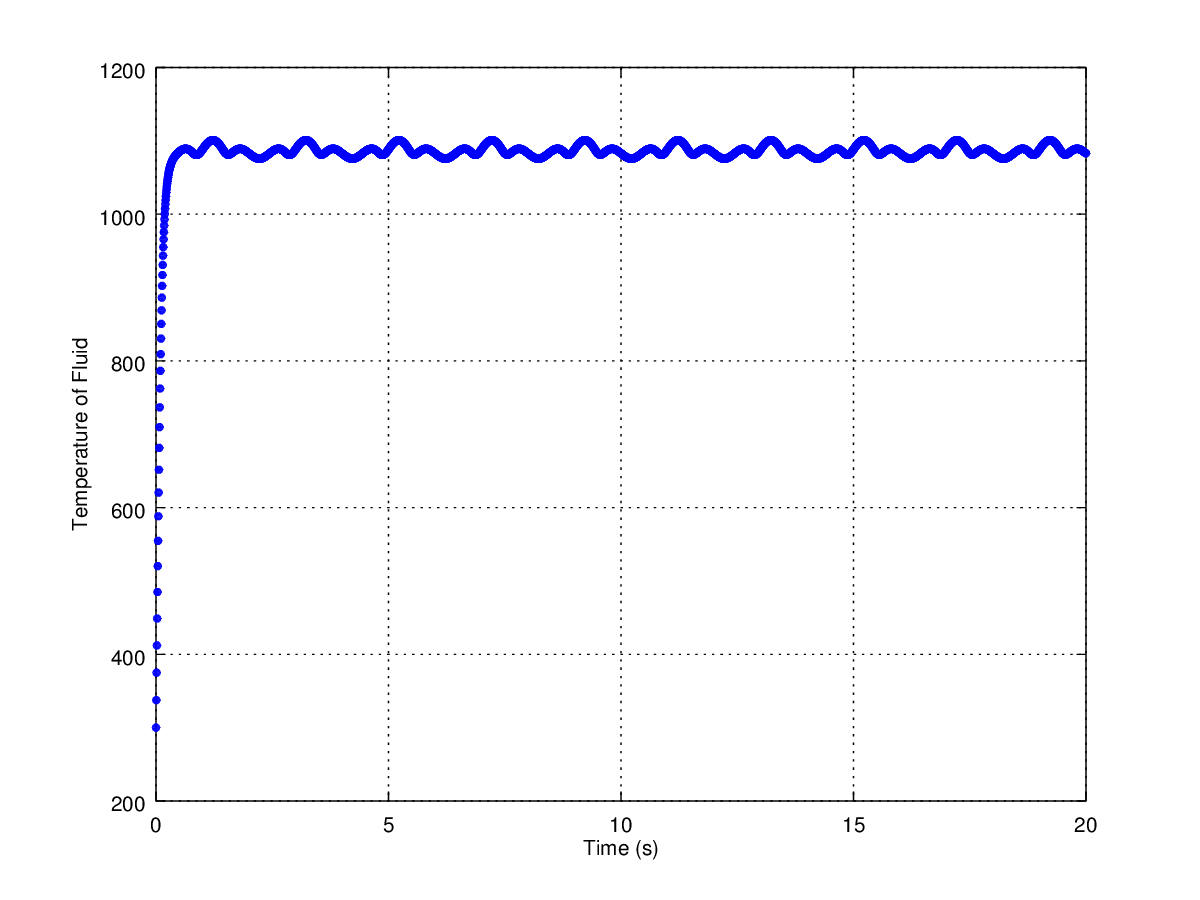
\includegraphics[scale=0.7]{task6fig}
\caption{Fluid Temperature Over Time}
\label{fig:fluidtemp}
\end{figure}
\end{center}


\section{Task 8: Heat Source Equation}
\subsection{Sampling the Heat Source Equation}
The solar heating function is given as
\[ Q(x,t) =
  \begin{cases}
    0       & \quad 0 <= x < 0.3\\
    200 sin(\pi \frac{x-0.3}{0.7}) | sin(\frac{\pi}{2} t) sin(\frac{3\pi}{2} t) |  & \quad x >= 0.3\\
  \end{cases}
\]

Sampling this equation at $x = 0.75$ for $0<=t<=10$ with a time step of $\Delta t = 0.1$ yeilds the results shown in Figure \ref{fig:task8fig1}.

\begin{center}
\begin{figure}
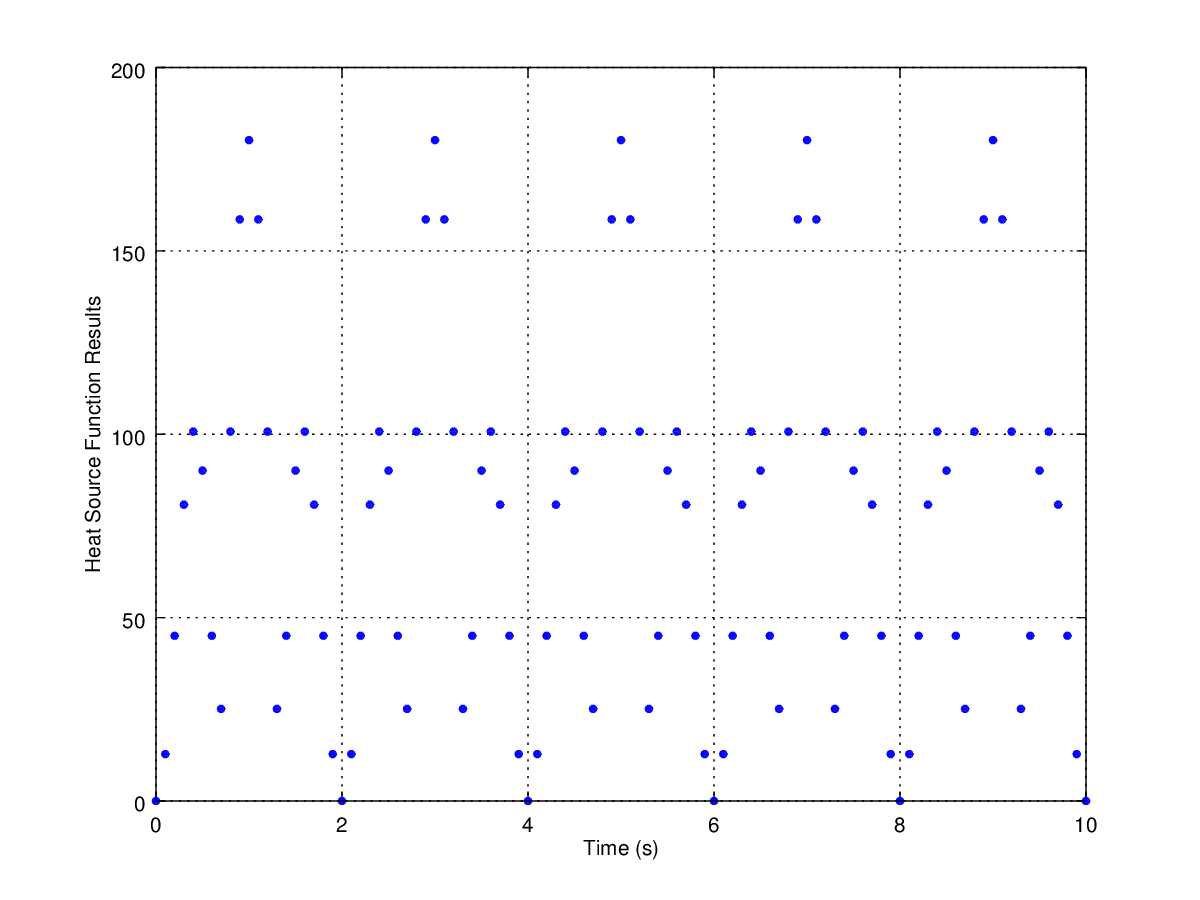
\includegraphics[scale=0.7]{task8fig1}
\caption{Heat Source Function Sampled at x = 0.75}
\label{fig:task8fig1}
\end{figure}
\end{center}


\subsection{Fourier Transformation}
Equation \ref{eq:fourier} shows the calculation of the discrete fourier transformation, where $h_k$ is the $k^{th}$ data sample and N is the total number of samples.
\begin{equation}
H(f_n) = \sum_{k=0}^{N-1} h_k e^\frac{2 \pi i k n}{N}
\label{eq:fourier}
\end{equation}

In this approximation, $n=0,...,N-1$ and $k=0,...,N-1$. \\
\subsubsection{Coefficients}
The coefficients of this transformation were calculated as follows, where H represents the fourier transform as calculated in Equation \ref{eq:fourier}. 
 \begin{equation}
 a_0 = \frac{1}{N} Re(H_1)
 \label{eq:a0}
 \end{equation}
 
 \begin{equation}
 a_k = \frac{2}{N} Re(H_{k+1})
 \label{eq:ak}
 \end{equation}
 
 \begin{equation}
 b_k = \frac{2}{N} Im(H_{k+1})
 \label{eq:ak}
 \end{equation}

These coefficients are plotted versus $\frac{k}{10}$ in Figures \ref{fig:akplot} and \ref{fig:bkplot}.

\begin{center}
\begin{figure}
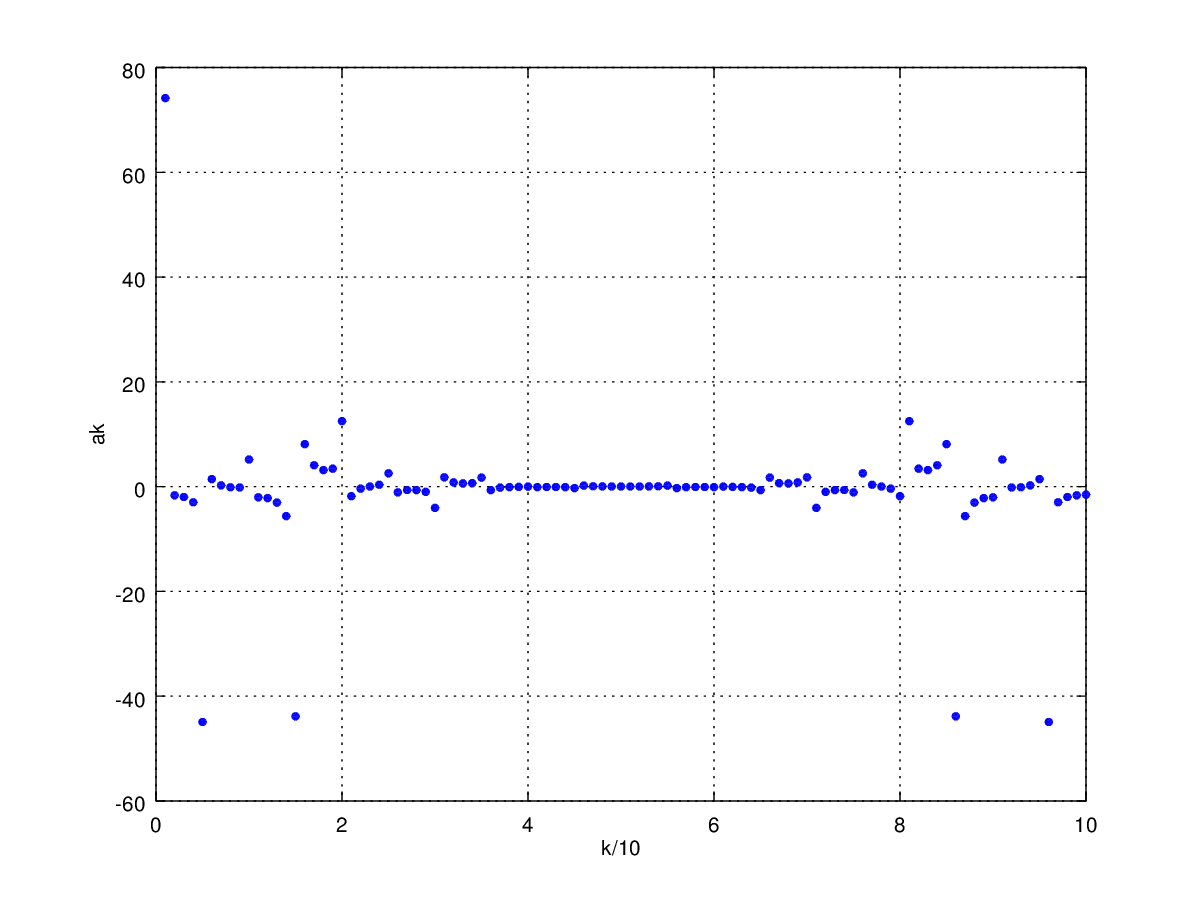
\includegraphics[scale=0.7]{akplot}
\caption{Coefficient ak}
\label{fig:akplot}
\end{figure}
\end{center}

\begin{center}
\begin{figure}
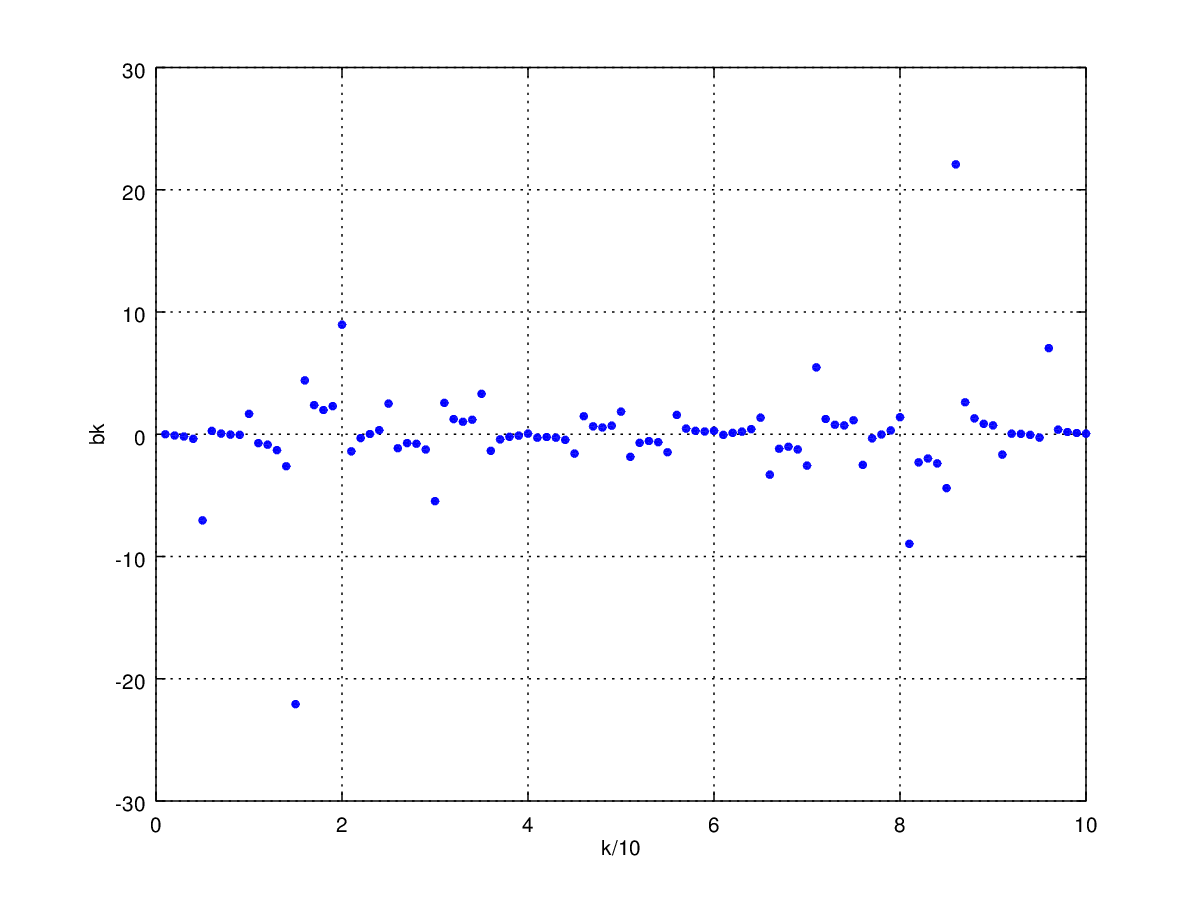
\includegraphics[scale=0.7]{bkplot}
\caption{Coefficient bk}
\label{fig:bkplot}
\end{figure}
\end{center}

\subsubsection{Power Spectrum}

The power spectrum for this transformation was computed using Equation \ref{eq:pk}, and is plotted in Figure \ref{fig:powerspectrum}. 

\begin{equation}
P_k = \frac{1}{2} \frac{a_k^2 + b_k^2}{N}
\label{eq:pk}
\end{equation}

\begin{center}
\begin{figure}
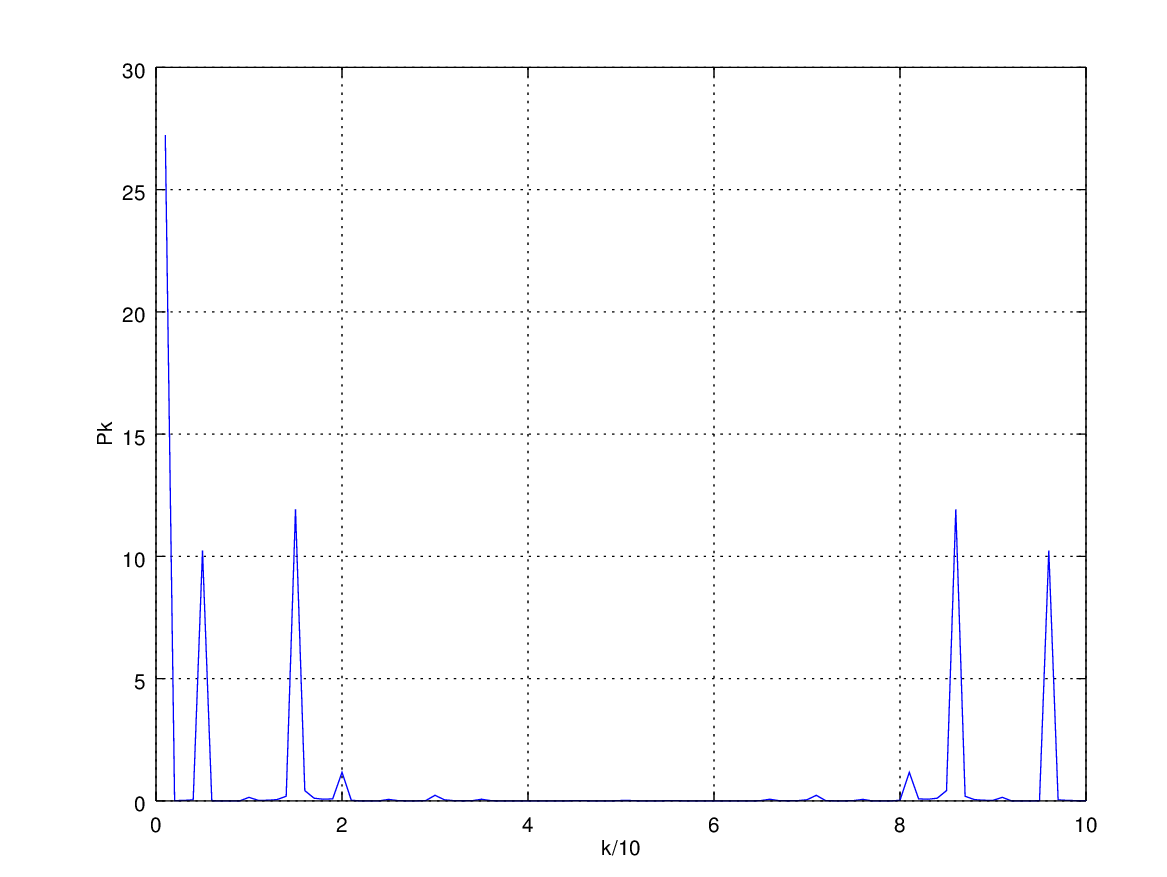
\includegraphics[scale=0.7]{Pkplot}
\caption{Power Spectrum}
\label{fig:powerspectrum}
\end{figure}
\end{center}

\section{Heat Stored in the Rod}
\subsection{Model}
The total heat stored in the rod at a given time is given in Equation \ref{eq:heat}. The Newton-Cotes approximation of this integral is given in Equation \ref{eq:newtoncotes}, where the integral is calculated over the interior points of the rod. 

\begin{equation}
H(t) = \int_0^L T(x,t) dx
\label{eq:heat}
\end{equation}

\begin{equation}
H(t) = \frac{x_{i+1}-x_i}{6} (T(x_{i+1},t) + 4T(x_i,t) + T(x_{i-1},t))
\label{eq:newtoncotes}
\end{equation}

\subsection{Results}
The results of Equation \ref{eq:newtoncotes} is plotted in Figure \ref{fig:totalheat}. Sampling this data set at $ t = 1.2$, we find the the heat stored in the rod is 294.222 Joules. The parameters used to determine this value are listed in Table \ref{task9param}. 

\begin{center}
\begin{figure}
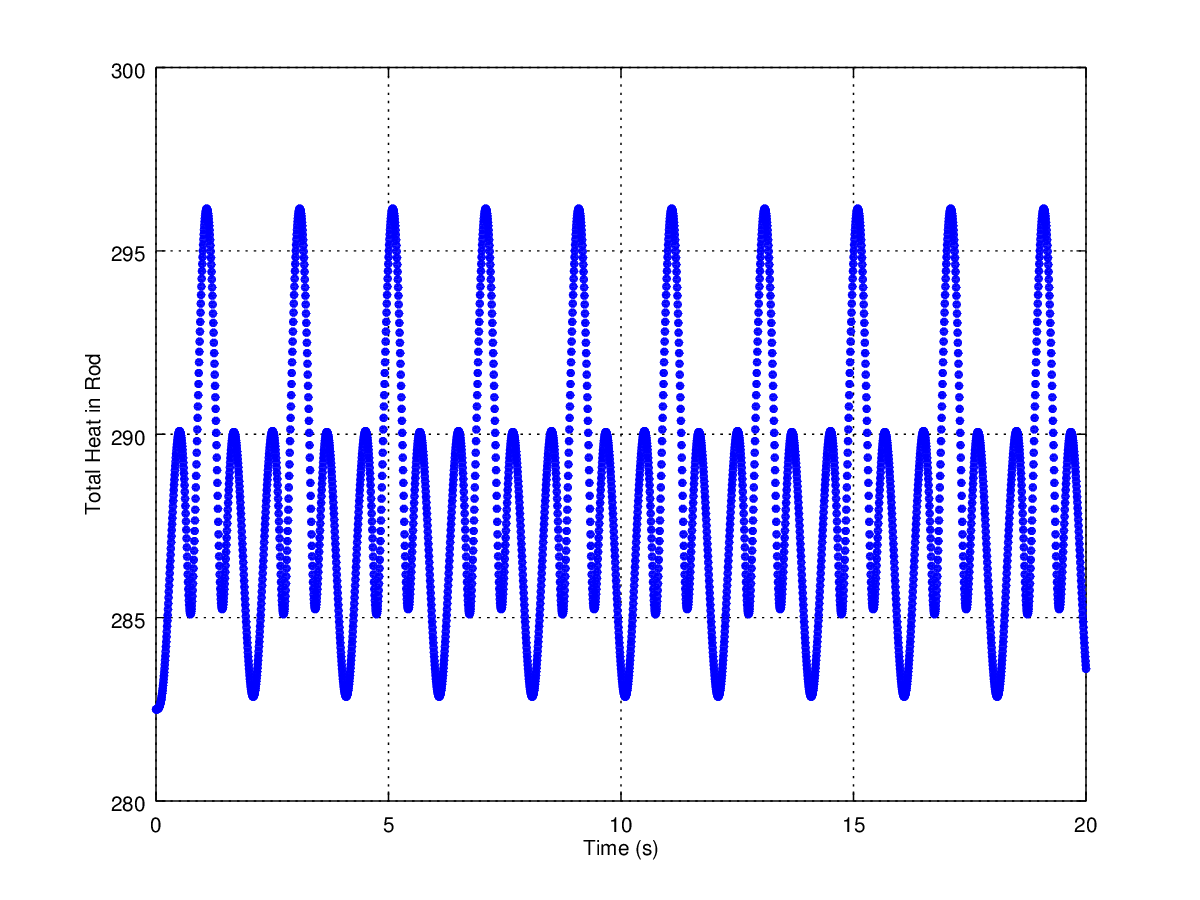
\includegraphics[scale=0.7]{task9plot}
\caption{Newton-Cotes Approximation of Heat Stored in Rod}
\label{fig:totalheat}
\end{figure}
\end{center}

\begin{table}[]
\centering
\caption{Task 9 Simulation Parameters}
\label{task9param}
\begin{tabular}{ll}
Parameter            & Value \\
$\Delta x$           & 0.05  \\
$\Delta t$           & 0.00625 
\end{tabular}
\end{table}
\end{document}